% --Relationen--

\subsection{Eigenschaften}

Wenn $R \subseteq A \times A$ eine Relation ist, dann ist $R$:
\begin{itemize}
\item \emph{symmetrisch}, falls für $(a, b) \in \mathbb{R}$ stets auch
  $(b, a) \in \mathbb{R}$ gilt, z.B. Rechwinkligkeit: wenn $a \bot b$ ist,
  dann ist $b \bot a$.
 \item \emph{antisymmetrisch} falls für $(a, b) \in \mathbb{R}$ und $(b, a) \in \mathbb{R}$  stets folgt: $a \equiv b$
 \item \emph{reflexiv} falls $(a, a) \in \mathbb{R}$ für alle $a$ in
   $A$ gilt, z.B. Parallelität: Jede Gerade ist zu sich selbst parallel
 \item \emph{transitiv} falls aus $(a, b) \in \mathbb{R}$ und $(b, c)
   \in \mathbb{R}$ folgt: $(a, c) \in \mathbb{R}$, z.B. Kleiner-Gleich
   ``$\leq$'': Wenn $a \leq b$ und $b \leq c$, dann gilt $a \leq c$.
\end{itemize}

\subsection{Beispiel einer Relation: Teilbarkeit}

Seien $a, b \in \mathbb{N}$. Dann ist $a$ \emph{Teiler von} $b$ genau dann, wenn
es ein $m \in \mathbb{N}$ gibt, so dass gilt: $a \cdot m = b$.

\paragraph{Bezeichnung:} $a \mid b$, $a \le_\tau b$

\paragraph{Beispiel:}
\begin{align*}
3 \mid 6,                    & \text{ denn }     3 \cdot 2 = 6    \\
n \mid 0,                    & \text{ für alle } n \in \mathbb{N} \\
n \le_\tau 0,                 & \text{ für alle } n \in \mathbb{N} \\
0 \mid 0, \text{ } 0 \nmid k & \text{ für alle } k \in \mathbb{N} \setminus \{0\} \text{ (es gibt }  m \in \mathbb{N}: 0 \cdot m = 0 \text{)} \\
1 \mid n,                    & \text{ für alle } n \in \mathbb{N} \\
\end{align*}

\paragraph{Bemerkung:}
$\le_\tau$ ist eine Relation über $\mathbb{N}$:

$\le_\tau $ ist eine Untermenge von $\mathbb{N} \times \mathbb{N}$.

$(a,b) $ ist ein Element von $\le_\tau$, wenn gilt $a \le_\tau b$.



\noindent $T_n$ sei die Menge der Teiler von $n (n \in \mathbb{N})$. \\ \indent {\bf Beispiel:} $T_{12} = \{ 1, 2, 3, 4, 6, 12 \}$ \\

\noindent Wir schränken $\le_\tau$ ein auf $T_n$: $\le_\tau \cap (T_n \times T_n) = \le_\tau^n$

\paragraph{Konvention:} wir schreiben $\le_\tau$ statt $\le_\tau \cap (A \times A)$, wenn klar ist, worauf sich $\le_\tau$ bezieht, also was $A$ ist. \\

\noindent $\mathbb{T}_n := (T_n, \le_\tau)$ heißt {\bf Teilerverband} von $n$.

\paragraph{Achtung:} $\mathbb{T}_n$ ist ein binäres Relat. Wir haben
bereits definiert, was $G (\mathbb{T}_n) = G (T_n, \le_\tau)$ ist:
$G (\mathbb{T}_n) = (T_n, \le_\tau, \sigma, \tau) \text{ mit:}$
\begin{align*}
\sigma (a, b) = a\\
\tau (a, b) = b\\
\forall (a, b) \in \le_\tau
\end{align*}

\paragraph{Beispiel:} $\mathbb{T}_6 = (T_6, \le_\tau), T_6 = { 1, 2, 3, 6}$

Teilerverband $G (\mathbb{T}_6) $:
\begin{figure}[h]
  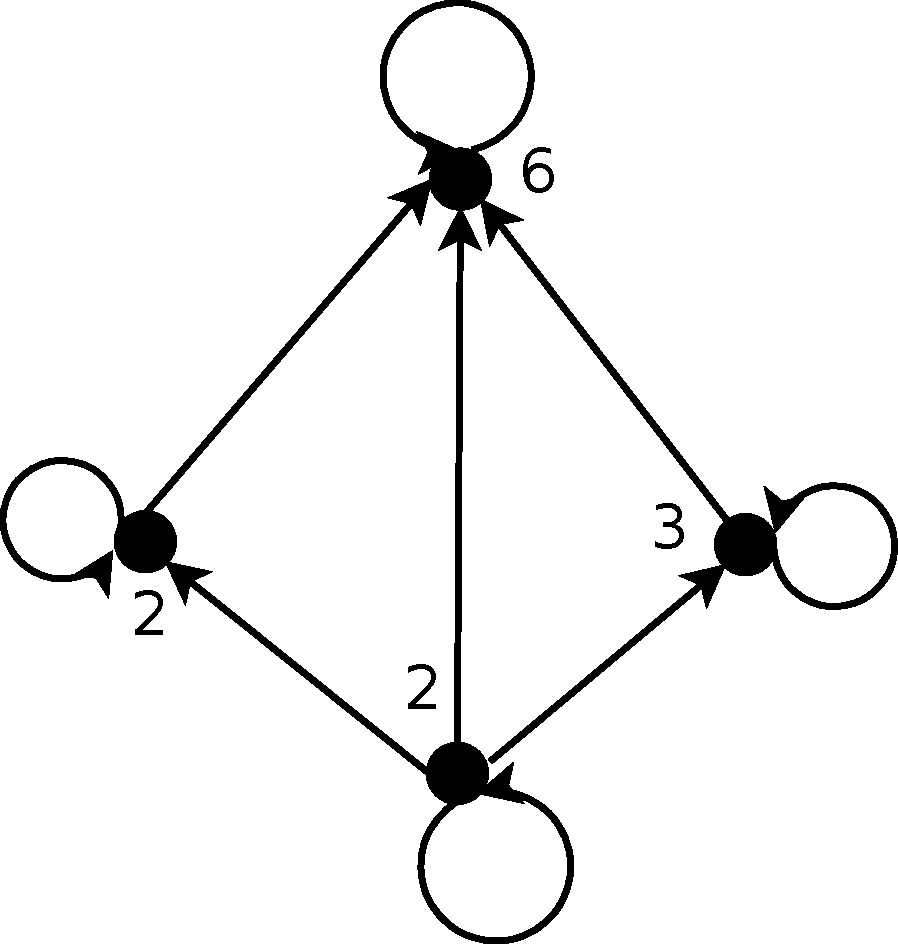
\includegraphics[scale=0.5,keepaspectratio=true]{../bilder/teilerverband.pdf}
\end{figure}

\noindent Ist $R$ eine Ordnung über $A$, dann ist $G (A, R)$ eine ungünstige Darstellung. \\ {\bf Besser:} Hasse-Diagramm:

$\le_\tau$ ist eine Relation auf $\mathbb{N}$, die gegeben ist durch: \\
$ \le_\tau = \{ (a, b) \in \le_\tau | \text{ für alle } c \in \mathbb{N} \text{ mit } a \le_\tau c \le_\tau b, (a, c), (c, b) \in \le_\tau \text{ gilt entweder } c = a \text{ oder } c = b \}$

\paragraph{Beispiel:}
\begin{itemize}
\item $(1, 6) \in \le_\tau$, aber $1 \le_\tau 2 \le_\tau 6$ und
                                 $1 \le_\tau 3 \le_\tau 6$,
  daraus folgt $(1, 6) \not\in\le_\tau$.
 \item $(2, 6) \in \le_\tau$ und für alle $c \in T_6$ mit $2 \le_\tau c \le_\tau 6$ gilt $c = 2$ oder $c = 6 \rightarrow (2, 6)$
\end{itemize}

\paragraph{Hassediagramm zu $\mathbb{T}_n$:}

Zeichne $G (T_n, \le_\tau)$, so dass der Knoten b über dem Knoten $a$
liegt, falls $(a, b) \in \le_\tau$ und zeichne Kanten $(a, b)$, also
$a$ ----- $b$ statt $a \longrightarrow b$. \\

\begin{figure}[h]
  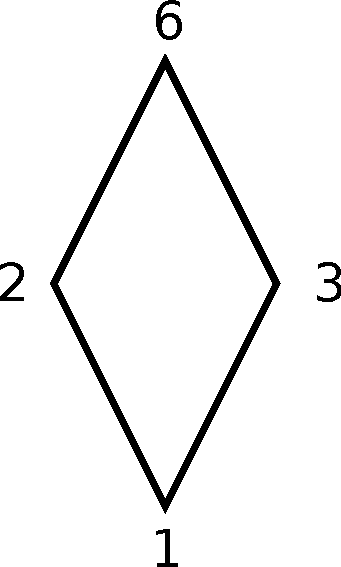
\includegraphics[scale=0.5,keepaspectratio=true]{../bilder/hassediagramm_von_6.pdf}
  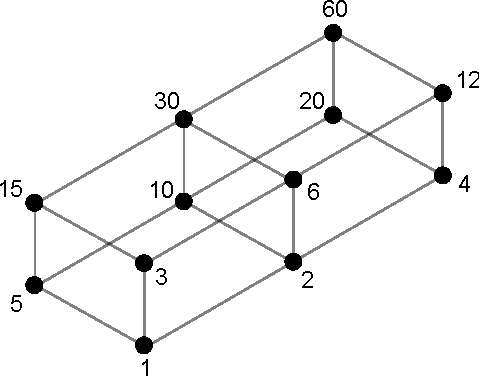
\includegraphics[keepaspectratio=true]{../bilder/hassediagramm_von_60.pdf}
  \caption{Hassediagramm vom Teilerverband 6 und 60}
\end{figure}

\subsection{Division mit Rest}

Die \emph{Division mit Rest} besagt, dass für 2 Zahlen $n$ und $m$
(ungleich 0) eindeutig bestimmte Zahlen $a$ und $b$ existieren für die gilt:
\begin{itemize}
\item $n = a * m + b$
\item $0 \le n < b$
\end{itemize}

Der Modulo berechnet den Rest $b$ der Division $n/m$. Schreibweise: $n \bmod a = b$

Beim Rechnen mit Modulo lassen sich häufig komplizierte Rechnung
vereinfachen/optimieren. Dabei gelten folgende Regeln:
\begin{align*}
  (a+b) \bmod n       &= ((a \bmod n) + (b \bmod n)) \bmod n \\
  (a-b) \bmod n       &= ((a \bmod n) - (b \bmod n)) \bmod n \\
  (a \cdot b) \bmod n &= ((a \bmod n) \cdot (b \bmod n)) \bmod n \\
\end{align*}

\paragraph{Beispiele}
\begin{align*}
  (3 \bmod 7)&= 3   \;\;   (17 \bmod 5)= 2   \;\;    (-9 \bmod 17)= 8 \\
  5^{167} \bmod 7 &= (5^2 \bmod 7) (5^3 \bmod 7)^{55} \bmod 7 \\
                 &= 4 \cdot (4 \cdot 5)^{55} \bmod 7 \\
                 &= 4 \cdot (-1)^{55} \bmod 7\\
                 &= -4 \bmod 7 = 3\\
\end{align*}

\subsection{Klassen von Relationen}

\begin{figure}[h]
  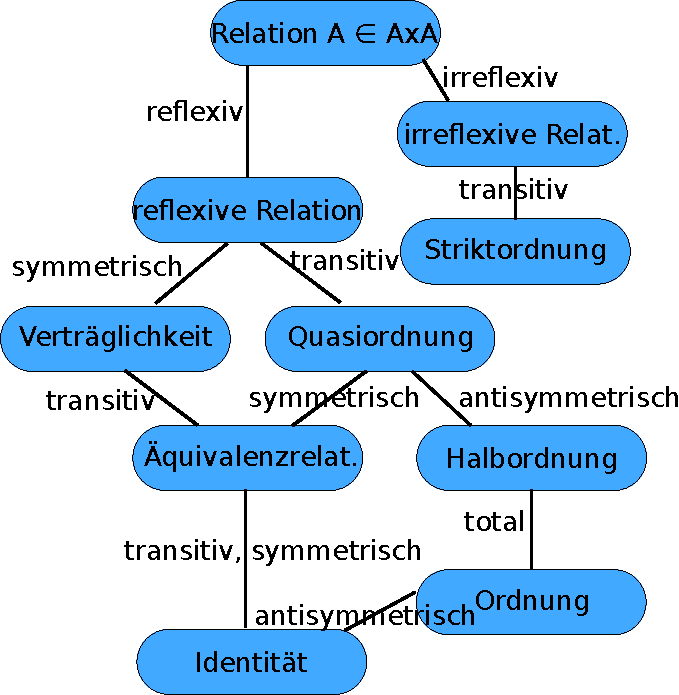
\includegraphics[scale=0.7,keepaspectratio=true]{../bilder/klassen_von_relationen.pdf}
  \caption{Arten von Relationen}
\end{figure}

\begin{itemize}
\item \emph{Totalordung} oder \emph{lineare Ordnung:} Für jedes
  beliebige 2 Elemente x,y der Grundmenge ($x \ne y$) ist stets die
  Relation xRy oder yRx erfüllt. \textbf{Beispiel:} $\le_\tau$ (Teiler
  von), $\le$ (kleiner gleich)
\item \emph{Quasiordnung:} für 3 Elemente $a,b,c$ der Grundmenge muss gelten:
  \begin{itemize}
  \item $a\lesssim a$ (Reflexivität)
  \item $a\lesssim b\lesssim c \implies a \lesssim c$ (Transivität)
  \end{itemize}
\item \emph{Äquivalenz(-relation)}  \textbf{Beispiel:} $=, \equiv$ (mod $n$)
\end{itemize}

\subsection{Äquivalenzrelation}
\begin{itemize}
\item teilt eine Menge $M$ restlos in nichtleere, elementfremde
  (disjunkte) Teilmengen (Äquivalenzklassen genannt)
  $[n] = \{n\} \; n \in N$
\item bei einer k-regulären Äquivalenzrelation sind alle Teilmengen
  gleich groß
\item die Menge der Äquivalenzrelationen von $M$ bildet eine Partition $N_{\subset}$
  von $M$ ($N_{\subset} = \{ [n] | n \in N\}$)
\end{itemize}



%%% Local Variables:
%%% mode: latex
%%% TeX-master: "script"
%%% End:
